\documentclass[11pt]{article}
\usepackage[margin=1in]{geometry}
\usepackage{amsmath,amssymb,booktabs,array,longtable}
\usepackage{graphicx}
\usepackage{epstopdf}      
\usepackage{hyperref}
\usepackage{enumitem}
\usepackage{titlesec}
\usepackage{float}

\begin{document}

\begin{center}
\Large\textbf{Shiv Nadar University Chennai}\\[2mm]
\end{center}

\renewcommand{\arraystretch}{1.4}

\begin{tabular}{|p{3.5cm}|p{8cm}|p{2cm}|}
\hline
Degree \& Branch & B.Tech Artificial Intelligence \& Data Science & Semester V\\ \hline
Subject Code \& Name & CS3807 -- Deep Learning Laboratory & AY: 2026--27\\ \hline
\end{tabular}

\vspace{3mm}

\begin{center}
\Large\textbf{Experiment 1}\\
\large\textbf{Implementation of a Single Layer Perceptron for Binary Classification}
\end{center}

%----------------------------------------------------------

\section*{1. Objective}

The objective of this experiment is to understand the concept of an artificial neuron and implement a Single Layer Perceptron from scratch for binary classification. Students will learn the perceptron learning algorithm, understand the importance of activation functions, visualize the learning process, and evaluate the classifier using a real-world dataset.

%----------------------------------------------------------

\section*{2. Background Theory}

An Artificial Neuron is the fundamental building block of a neural network. It receives one or more input features, multiplies them by corresponding weights, adds a bias term, and applies an activation function to determine the output.

The Single Layer Perceptron is the earliest supervised learning algorithm capable of solving linearly separable binary classification problems.

\subsection*{Mathematical Formulation}

Weighted Sum

\[
z=\mathbf{w}^{T}\mathbf{x}+b
\]

where

\begin{itemize}
\item $\mathbf{x}$ : Input vector
\item $\mathbf{w}$ : Weight vector
\item $b$ : Bias
\item $z$ : Linear combination
\end{itemize}

Prediction

\[
\hat y=f(z)
\]

Weight Update Rule

\[
\mathbf{w}_{new}
=
\mathbf{w}_{old}
+
\eta
(y-\hat y)
\mathbf{x}
\]

Bias Update

\[
b_{new}
=
b_{old}
+
\eta
(y-\hat y)
\]

where $\eta$ denotes the learning rate.

%----------------------------------------------------------

\section*{3. Activation Functions}

An activation function determines the output of a neuron based on the weighted sum of its inputs. It introduces non-linearity, enabling neural networks to learn complex patterns. Although the perceptron uses only the Step Activation Function, modern deep learning models employ differentiable activation functions for efficient optimization through backpropagation.

\subsection*{Step Activation Function}

\[
f(z)=
\begin{cases}
1,&z\ge0\\
0,&z<0
\end{cases}
\]

The Step Activation Function produces a binary output and is therefore suitable only for linearly separable binary classification problems.

\begin{center}
\begin{tabular}{|p{2.5cm}|p{3cm}|p{6cm}|}
\hline
\textbf{Activation} & \textbf{Output Range} & \textbf{Typical Applications}\\
\hline
Step & $\{0,1\}$ & Classical Perceptron\\
\hline
Sigmoid & $(0,1)$ & Binary Classification Output Layer\\
\hline
Tanh & $(-1,1)$ & Hidden Layers (Traditional Networks)\\
\hline
ReLU & $[0,\infty)$ & Hidden Layers in CNNs and MLPs\\
\hline
Leaky ReLU & $(-\infty,\infty)$ & Avoiding Dying ReLU\\
\hline
Softmax & $(0,1)$ & Multi-class Classification Output Layer\\
\hline
\end{tabular}
\end{center}

\textbf{Note:} This experiment uses only the Step Activation Function. The remaining activation functions will be studied in subsequent experiments involving Multilayer Perceptrons and Deep Neural Networks.

%----------------------------------------------------------

\section*{4. Dataset Description}

\textbf{Dataset:} Banknote Authentication Dataset

\textbf{Source:} UCI Machine Learning Repository

\textbf{Download Link:}

\url{https://archive.ics.uci.edu/dataset/267/banknote+authentication}

\begin{center}
\begin{tabular}{|l|l|}
\hline
Instances & 1372\\
\hline
Features & 4 Numerical Features\\
\hline
Classes & 2\\
\hline
Missing Values & None\\
\hline
Task & Binary Classification\\
\hline
\end{tabular}
\end{center}

\textbf{Feature Description}

\begin{itemize}
\item Variance
\item Skewness
\item Curtosis
\item Entropy
\end{itemize}

Target Class

\begin{itemize}
\item 0 -- Authentic Banknote
\item 1 -- Forged Banknote
\end{itemize}

%----------------------------------------------------------

\section*{5. Experimental Procedure}

\textbf{Task 1: Dataset Exploration}

\begin{itemize}
\item Load the dataset.
\item Display the first five samples.
\item Determine dataset dimensions.
\item Identify missing values.
\item Display descriptive statistics.
\end{itemize}

\vspace{2mm}

\textbf{Task 2: Exploratory Data Analysis}

Generate

\begin{itemize}
\item Histograms
\item Correlation Heatmap
\item Scatter Plot
\item Boxplots
\end{itemize}

\vspace{2mm}

\textbf{Task 3: Data Preprocessing}

\begin{itemize}
\item Normalize all numerical features.
\item Split the dataset into Training (80\%) and Testing (20\%).
\end{itemize}

\vspace{2mm}

\textbf{Task 4: Perceptron Implementation}

Implement from scratch

\begin{itemize}
\item Weight Initialization
\item Bias Initialization
\item Step Activation Function
\item Forward Propagation
\item Perceptron Learning Rule
\end{itemize}

\vspace{2mm}

\textbf{Task 5: Model Training}

Display

\begin{itemize}
\item Epoch Number
\item Misclassified Samples
\item Updated Weights
\item Updated Bias
\end{itemize}

\vspace{2mm}

\textbf{Task 6: Model Evaluation}

Compute

\begin{itemize}
\item Accuracy
\item Precision
\item Recall
\item F1-score
\item Confusion Matrix
\end{itemize}

%----------------------------------------------------------

\section*{6. Source Code}

The complete implementation (data loading, EDA, preprocessing, the from-scratch Perceptron class, training loop, evaluation, and learning-rate comparison) is available at the following GitHub repository:

\begin{center}
\url{https://github.com/PolarFox08/Deep-Learning-Lab/blob/main/Deep%20Learning%20Lab%201/DL_Lab_1_Perceptron.ipynb}
\end{center}

%----------------------------------------------------------

\section*{7. Experimental Results}

The perceptron was trained for 50 epochs with a learning rate of $\eta = 0.01$ on the standardized/normalized features, using an 80:20 train--test split (1097 training samples, 275 testing samples).

During training, the number of misclassified samples per epoch dropped sharply from 166 (epoch 1) to under 20 within the first 10 epochs, and then oscillated in a low range (roughly 14--26 misclassified samples) for the remaining epochs without reaching exactly zero. This indicates the model did not achieve perfect convergence, which is expected since the Banknote Authentication dataset is only \emph{approximately} linearly separable (as seen in the EDA boxplots and scatter plots, where curtosis and entropy show considerable overlap between classes).

The final trained model (epoch 50) had:

\begin{itemize}
\item \textbf{Weights:} $[-0.181,\ -0.180,\ -0.208,\ 0.006]$ (variance, skewness, curtosis, entropy)
\item \textbf{Bias:} $0.240$
\end{itemize}

On the held-out test set, the model achieved:

\begin{center}
\begin{tabular}{|l|c|}
\hline
\textbf{Metric} & \textbf{Value}\\
\hline
Accuracy & 0.9891\\
\hline
Precision & 1.0000\\
\hline
Recall & 0.9764\\
\hline
F1-score & 0.9880\\
\hline
\end{tabular}
\end{center}

A precision of 1.0000 indicates zero false positives -- every banknote predicted as authentic was genuinely authentic. The small gap between precision and recall (0.9764) indicates a few forged notes were misclassified as authentic (false negatives), which is what pulled the F1-score slightly below 1.

\textbf{Comparison with Scikit-learn's Perceptron}

\begin{center}
\begin{tabular}{|l|c|}
\hline
\textbf{Implementation} & \textbf{Test Accuracy}\\
\hline
From-scratch Perceptron & 0.98909\\
\hline
Scikit-learn Perceptron & 0.97818\\
\hline
\end{tabular}
\end{center}

The from-scratch implementation slightly outperformed scikit-learn's built-in \texttt{Perceptron} on this split. This is not evidence that the manual implementation is fundamentally superior -- the two are not doing identical computations. Scikit-learn's \texttt{Perceptron} shuffles the training data at the start of every epoch by default and applies an early-stopping criterion (\texttt{tol}, \texttt{n\_iter\_no\_change}), whereas the from-scratch version processes samples in a fixed order for a fixed 50 epochs. These implementation-level differences lead to slightly different final decision boundaries, so small accuracy differences of a point or two in either direction are expected on a small (275-sample) test set, not a sign of error.

%----------------------------------------------------------

\section*{8. Generated Plots with Interpretation}

\subsection*{8.1 Feature Histograms}
\begin{figure}[H]
\centering
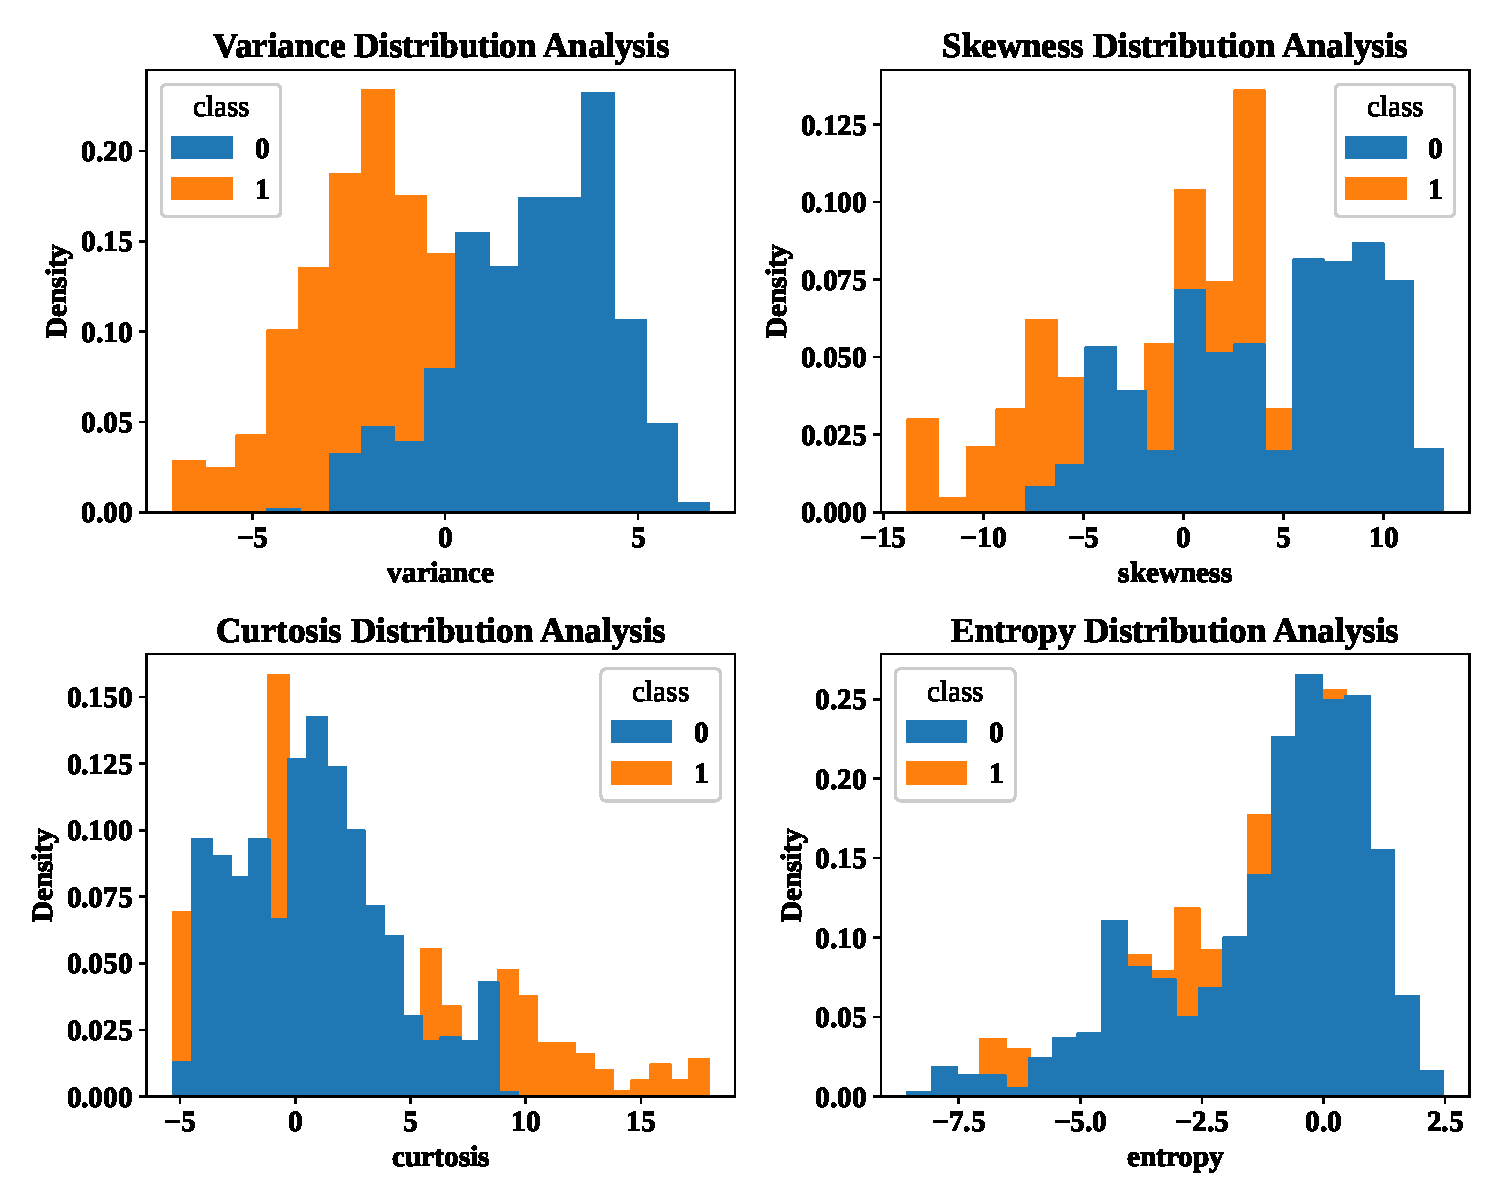
\includegraphics[width=0.85\textwidth]{feature_histogram.eps}
\caption{Distribution of each feature (variance, skewness, curtosis, entropy) split by class.}
\end{figure}
\textbf{Interpretation:} % TODO: write 2--3 sentences
It is clear from the histogram plots that variance is the only symmetric and uniform distribution, with noticeable separation between the 2 classes. Curtosis and Entropy are extremely skewed and hence have extreme outlier values. The skewness distribution isn't as skewed as curtosis or entropy but still is slightly negatively skewed.

\subsection*{8.2 Correlation Heatmap}
\begin{figure}[H]
\centering
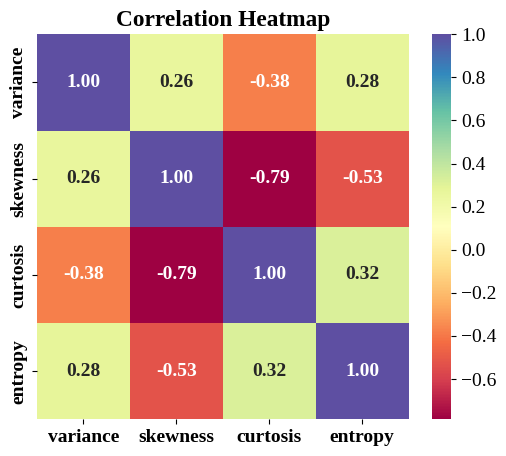
\includegraphics[width=0.6\textwidth]{correlation_heatmap.png}
\caption{Pairwise correlation between the four input features.}
\end{figure}
\textbf{Interpretation:} % TODO: write 2--3 sentences
Skewness and Curtosis are highly negatively correlated meaning curtosis decreases as skewness increases. At the same time there is a significant amount of negative correlation between skewness and entropy too.
\subsection*{8.3 Scatter Plot}
\begin{figure}[H]
\centering
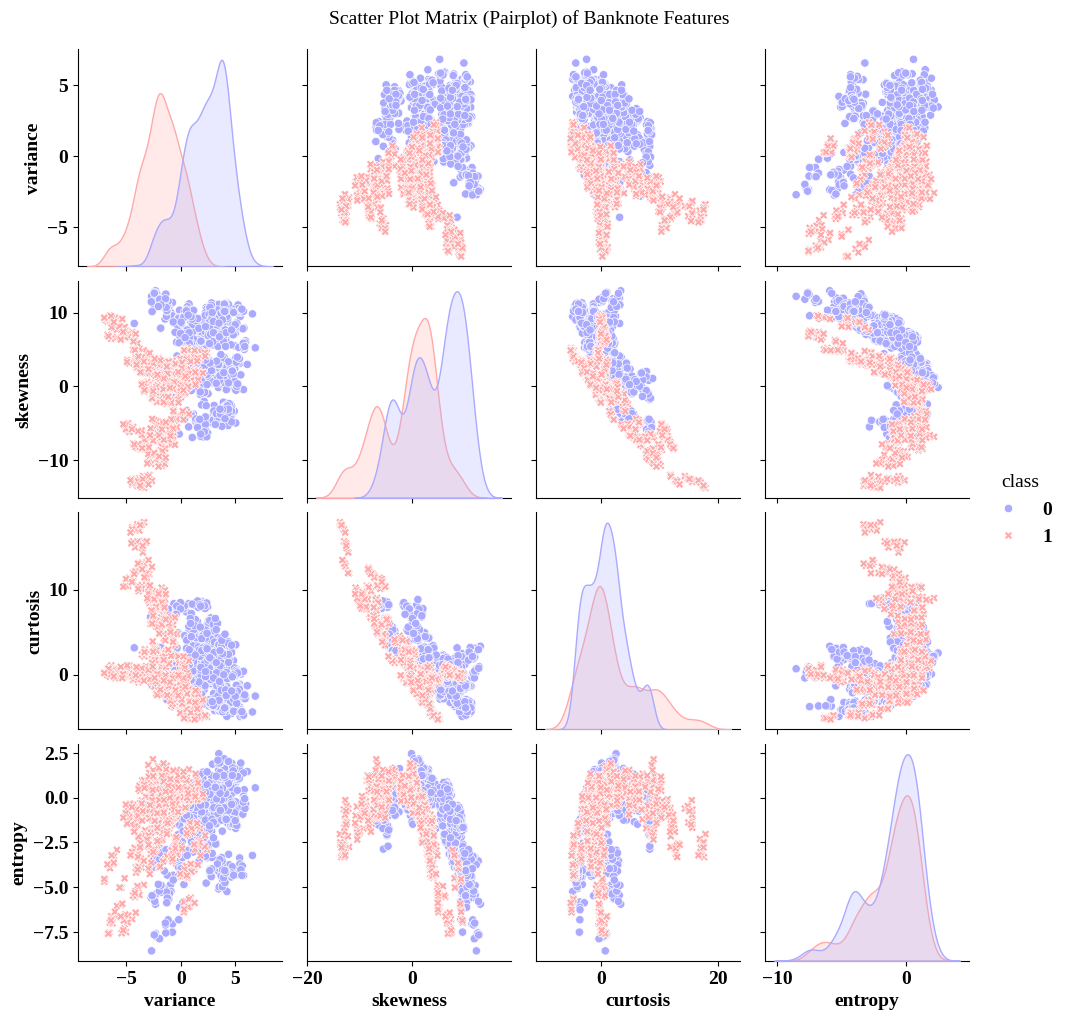
\includegraphics[width=0.85\textwidth]{scatter_plot.png}
\caption{Pairwise scatter plot / scatter matrix of features colored by class.}
\end{figure}
\textbf{Interpretation:} % TODO: write 2--3 sentences
All the pair plots have been generated in 4x4 matrix, each color-separated by the class labels. Most of the scatter plots have less overlap between both classes, while some have almost none. Hence we can conclude that the data is linearly separable !

\subsection*{8.4 Box-plots}
\begin{figure}[H]
\centering
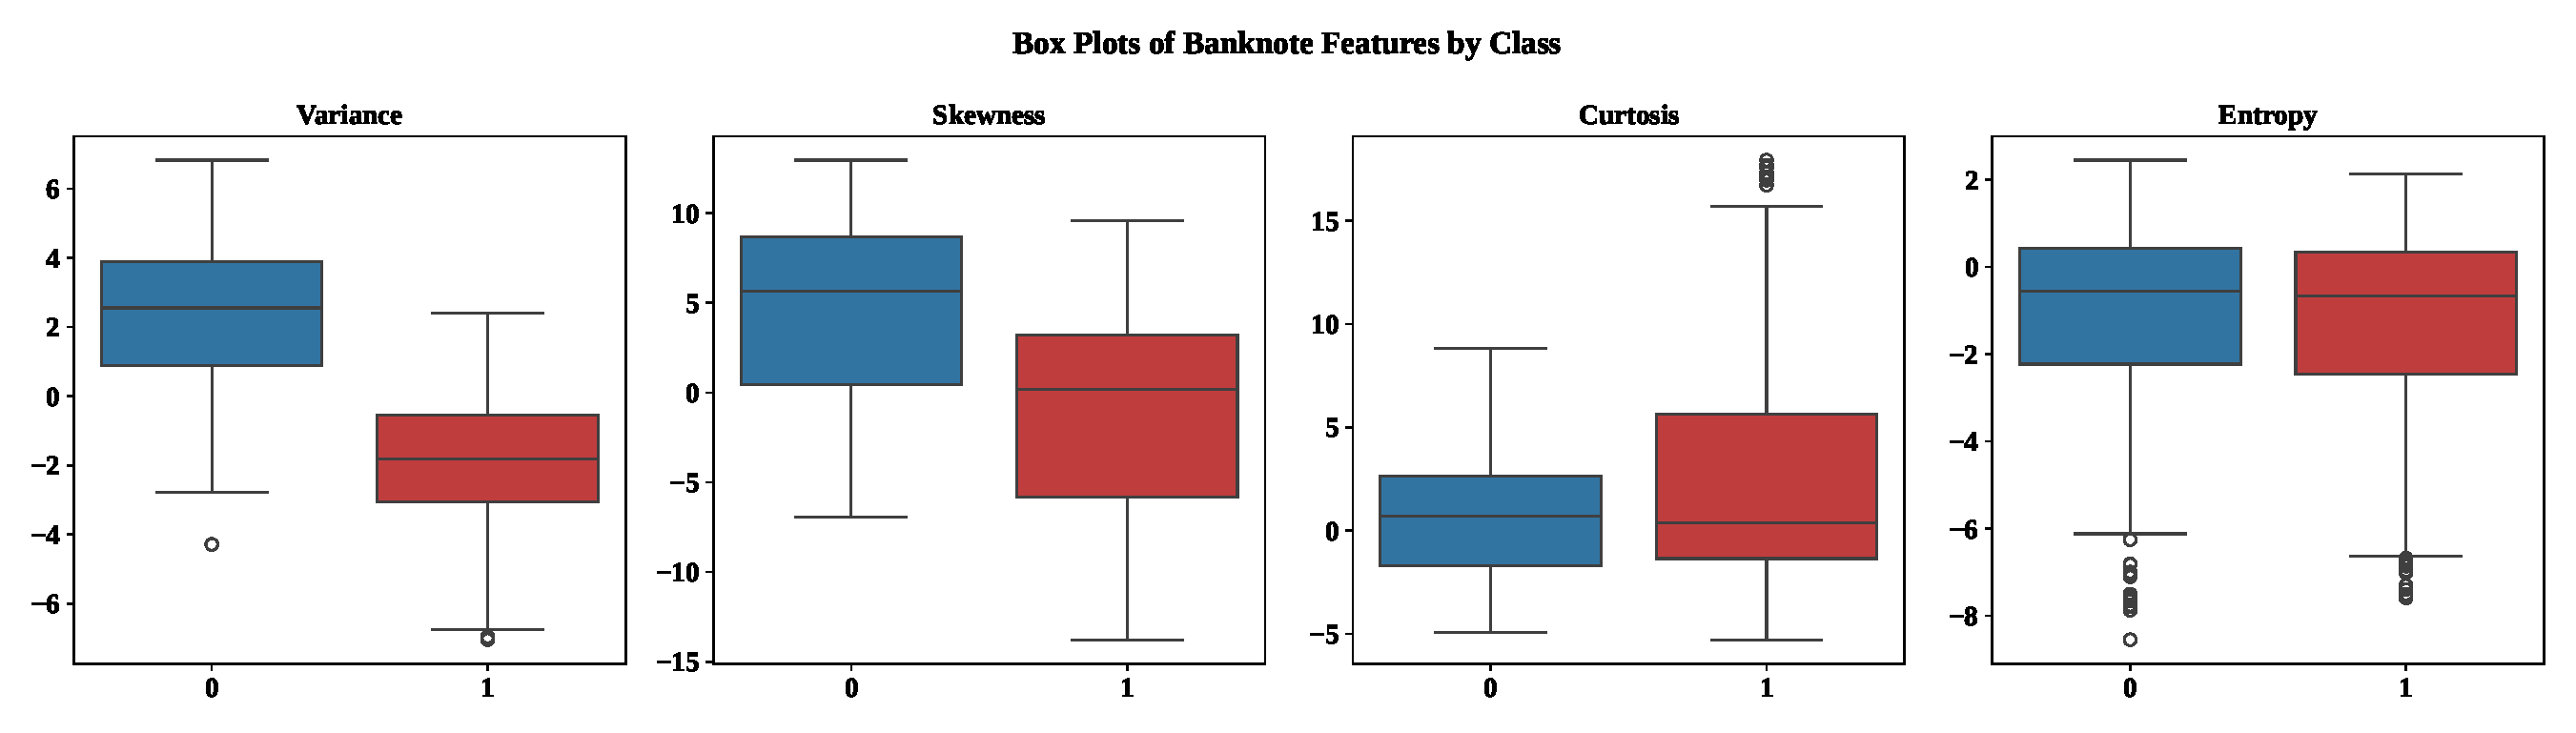
\includegraphics[width=0.85\textwidth]{boxplots.eps}
\caption{Box-plots of each feature grouped by class.}
\end{figure}
\textbf{Interpretation:} % TODO: write 2--3 sentences
There is no overlapping between genuine and forged notes when it comes to variances while skewness has somewhat of an overlap. However the notes cannot be separated by looking at curtosis and entropy as both classes have almost full overlap in both features.

\subsection*{8.5 Training Error vs Epoch}
\begin{figure}[H]
\centering
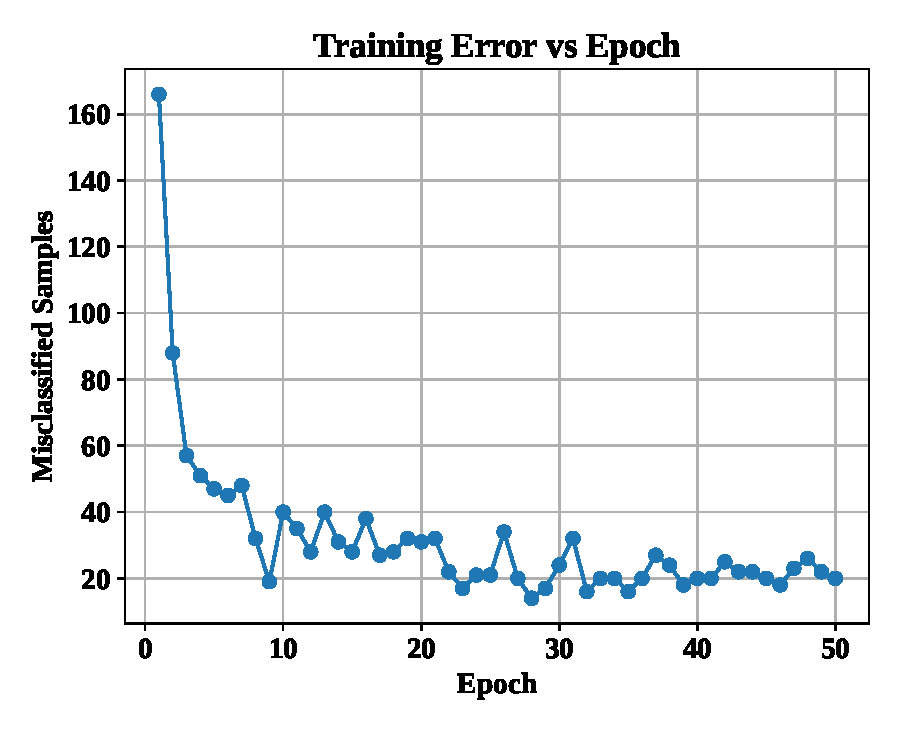
\includegraphics[width=0.7\textwidth]{training_error.eps}
\caption{Number of misclassified training samples per epoch.}
\end{figure}
\textbf{Interpretation:} % TODO: write 2--3 sentences
We observe the error (misclassified samples) reduce drastically after the first few epochs. The error of the perceptron later "stabilized" when about 30 epochs had been reached.

\subsection*{8.6 Weight Evolution}
\begin{figure}[H]
\centering
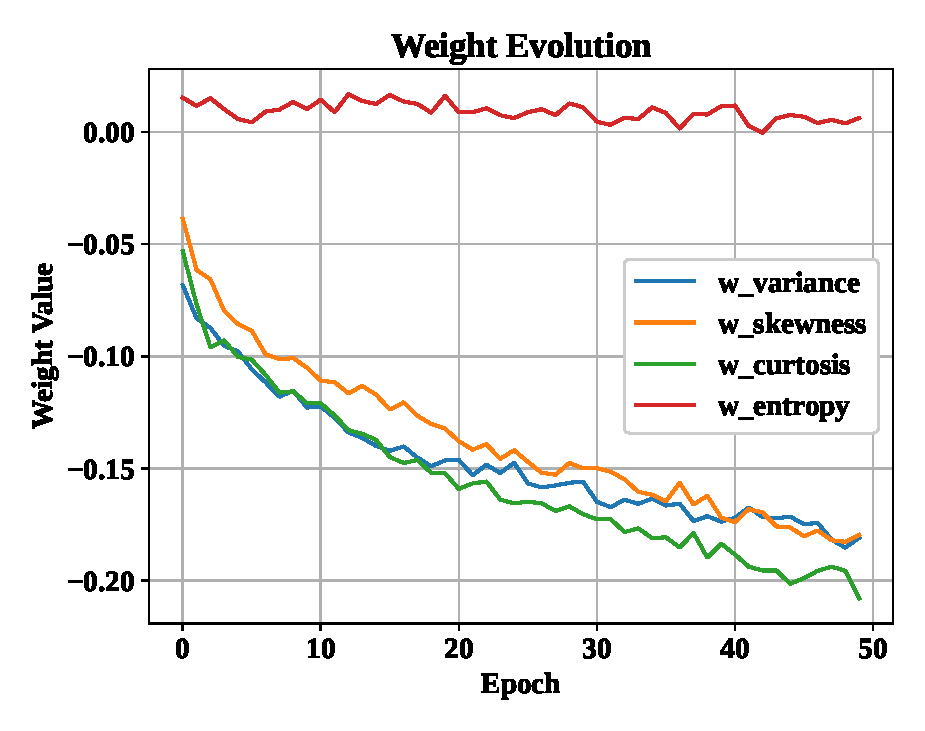
\includegraphics[width=0.7\textwidth]{weight_evolution.eps}
\caption{Evolution of the four feature weights across training epochs.}
\end{figure}
\textbf{Interpretation:} % TODO: write 2--3 sentences
Weight values changed abruptly during the initial epochs. However the weight values later flat line when our model was able to find a good enough decision boundary between the target classes as the epochs grew.

\subsection*{8.7 Bias Evolution}
\begin{figure}[H]
\centering
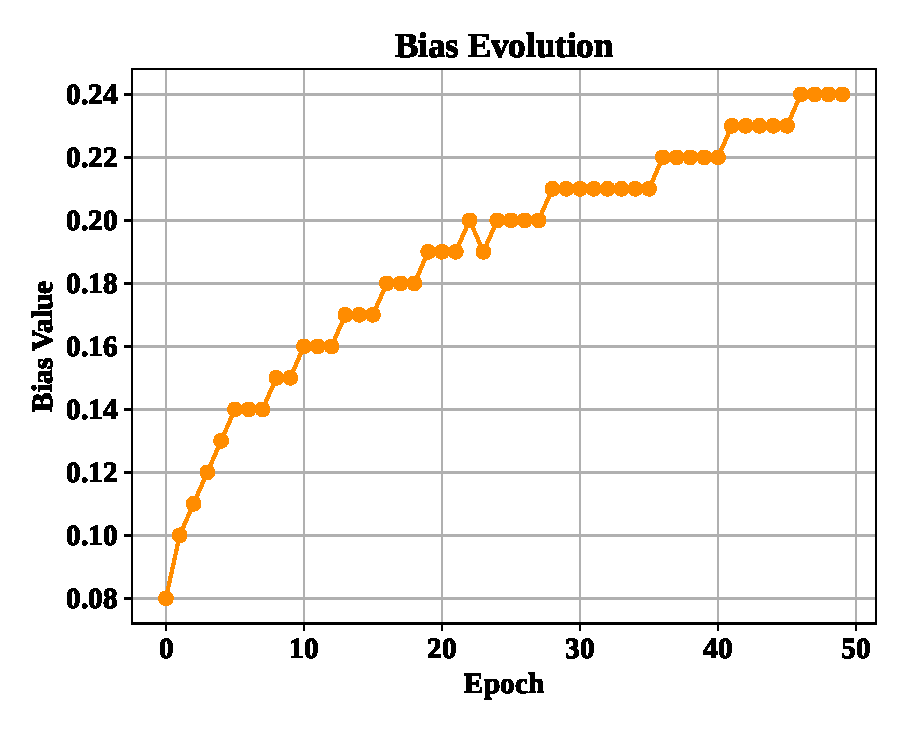
\includegraphics[width=0.7\textwidth]{bias_evolution.eps}
\caption{Evolution of the bias term across training epochs.}
\end{figure}
\textbf{Interpretation:} % TODO: write 2--3 sentences
The bias value kept increasing significantly in the initial epochs. In the later epochs the increase wasn't as huge as the initial increase but the values still were constantly rising.

\subsection*{8.8 Confusion Matrix}
\begin{figure}[H]
\centering
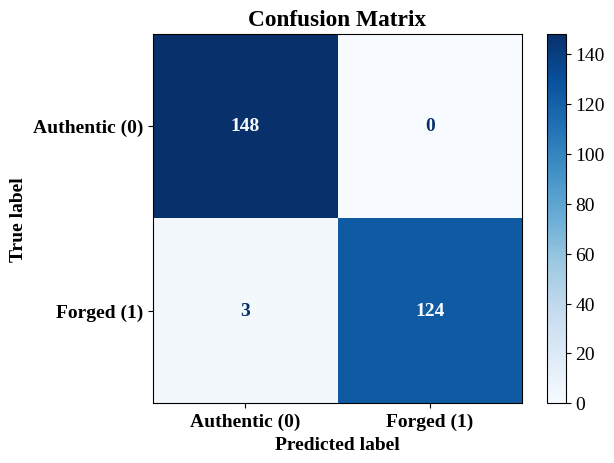
\includegraphics[width=0.5\textwidth]{confusion_matrix.png}
\caption{Confusion matrix on the test set.}
\end{figure}
\textbf{Interpretation:} % TODO: write 2--3 sentences
Only 3 samples were wrongly classified as authentic bills, hence the slight reduction in accuracy. However, all the authentic bills were predicted correctly,hence the model has 100\% precision.

\subsection*{8.9 Learning Rate Comparison}
\begin{figure}[H]
\centering
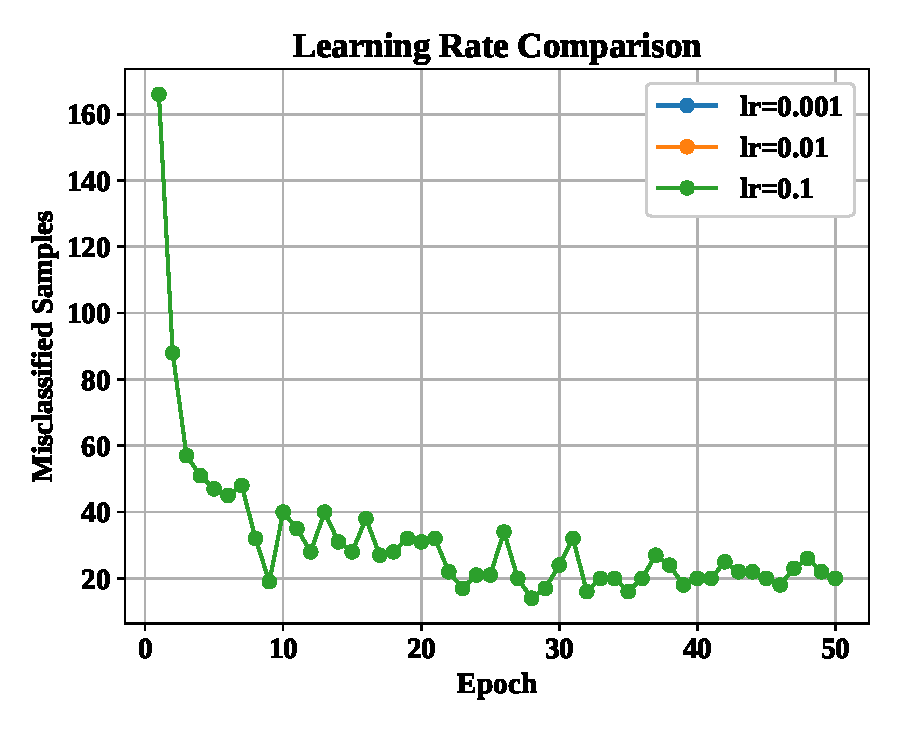
\includegraphics[width=0.7\textwidth]{learning_rate_comparison.eps}
\caption{Training error curves for $\eta = 0.001, 0.01, 0.1$.}
\end{figure}
\textbf{Interpretation:} % TODO: write 2--3 sentences
All three curves end up on top of each other. This is because at every epoch the same samples were misclassified as they had the same sign, even though they had different learning rates.

\subsection*{8.10 Decision Boundary (Optional)}
\begin{figure}[H]
\centering
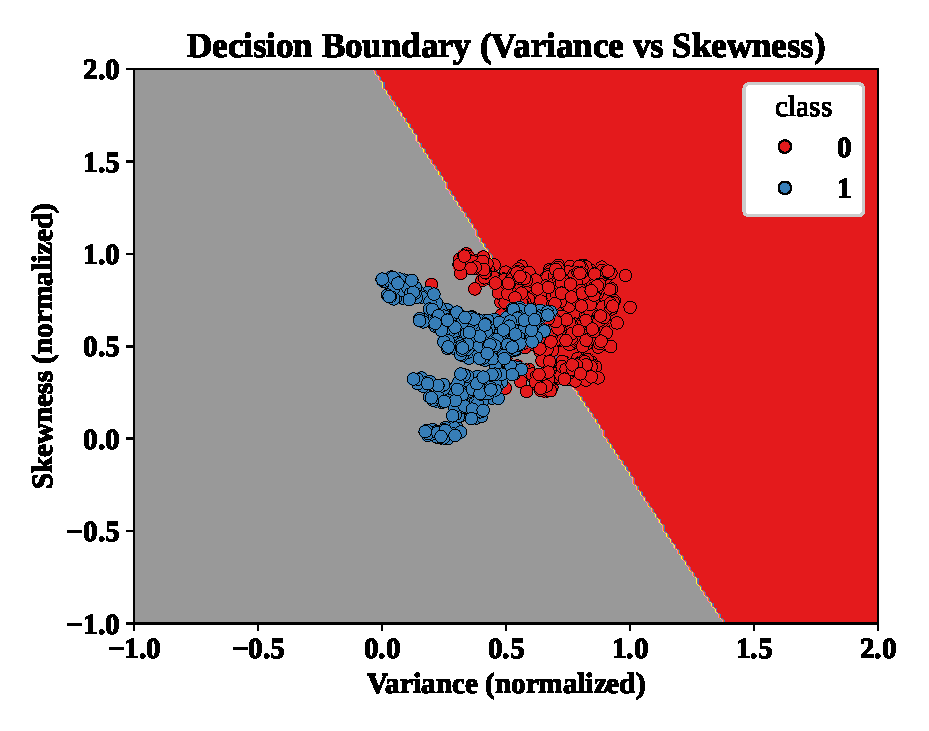
\includegraphics[width=0.7\textwidth]{decision_boundary.eps}
\caption{Decision boundary using two selected features (variance, skewness).}
\end{figure}
\textbf{Interpretation:} % TODO: write 2--3 sentences
Variance and Skewness features were chosen and a linear decision boundary was drawn on their scatter plot. But since they are not linearly separable, it wasn't possible to separate both features using a linear boundary.
%----------------------------------------------------------

\section*{9. Performance Tables}

\textbf{Training Summary}

\begin{center}
\begin{tabular}{|p{6cm}|p{7cm}|}
\hline
Dataset Size & 1372 samples\\
\hline
Train/Test Split & 1097 / 275 (80\% / 20\%)\\
\hline
Learning Rate & 0.01\\
\hline
Epochs & 50 (did not fully converge to zero error)\\
\hline
Final Weights & $[-0.181,\ -0.180,\ -0.208,\ 0.006]$\\
\hline
Final Bias & 0.240\\
\hline
Accuracy & 0.9891\\
\hline
Precision & 1.0000\\
\hline
Recall & 0.9764\\
\hline
F1-score & 0.9880\\
\hline
\end{tabular}
\end{center}

\vspace{3mm}

\textbf{Epoch-wise Learning (selected epochs)}

\begin{center}
\begin{tabular}{|c|c|c|c|c|}
\hline
Epoch & Errors & Weight 1 (variance) & Weight 2 (skewness) & Bias\\
\hline
1  & 166 & $-0.068$ & $-0.039$ & $0.080$\\
\hline
10 & 40  & $-0.123$ & $-0.105$ & $0.150$\\
\hline
20 & 31  & $-0.146$ & $-0.132$ & $0.190$\\
\hline
30 & 24  & $-0.156$ & $-0.150$ & $0.210$\\
\hline
40 & 20  & $-0.174$ & $-0.172$ & $0.220$\\
\hline
50 & 20  & $-0.181$ & $-0.180$ & $0.240$\\
\hline
\end{tabular}
\end{center}

% ==============================================================================
% PERCEPTRON LEARNING ALGORITHM SECTION
% ==============================================================================

\section*{10. Perceptron Learning Algorithm for AND, OR, and NOT Gates}

\textbf{Overview}

This section presents the step-by-step training process of a single-layer Perceptron learning the \textbf{AND}, \textbf{OR}, and \textbf{NOT} logic gates. Weight updates occur online whenever a sample is misclassified using a learning rate of $\eta = 0.1$.

\vspace{3mm}

% ------------------------------------------------------------------------------
% 1. AND GATE
% ------------------------------------------------------------------------------
\subsection*{AND Gate}

\textbf{Step-by-Step Weight Update Logs}

\begin{center}
\begin{tabular}{|c|c|c|c|c|c|c|}
\hline
Epoch & Update \# & Sample ($x$) & Target ($y$) & Predicted ($\hat{y}$) & New Weights ($w_1, w_2$) & New Bias ($b$)\\
\hline
1 & 1 & $[0,\ 0]$ & 0 & 1 & $[0.000,\ 0.000]$ & $-0.100$\\
\hline
1 & 2 & $[1,\ 1]$ & 1 & 0 & $[0.100,\ 0.100]$ & $0.000$\\
\hline
2 & 3 & $[0,\ 0]$ & 0 & 1 & $[0.100,\ 0.100]$ & $-0.100$\\
\hline
2 & 4 & $[0,\ 1]$ & 0 & 1 & $[0.100,\ 0.000]$ & $-0.200$\\
\hline
2 & 5 & $[1,\ 1]$ & 1 & 0 & $[0.200,\ 0.100]$ & $-0.100$\\
\hline
3 & 6 & $[0,\ 1]$ & 0 & 1 & $[0.200,\ 0.000]$ & $-0.200$\\
\hline
3 & 7 & $[1,\ 0]$ & 0 & 1 & $[0.100,\ 0.000]$ & $-0.300$\\
\hline
3 & 8 & $[1,\ 1]$ & 1 & 0 & $[0.200,\ 0.100]$ & $-0.200$\\
\hline
\end{tabular}
\end{center}

\vspace{3mm}

\textbf{AND Gate Summary}

\begin{center}
\begin{tabular}{|p{6cm}|p{7cm}|}
\hline
Convergence Status & Converged at Epoch 4\\
\hline
Total Updates & 8 updates\\
\hline
Final Weights & $[0.200,\ 0.100]$\\
\hline
Final Bias & $-0.200$\\
\hline
\end{tabular}
\end{center}

\begin{figure}[htbp]
    \centering
    % TODO: Replace 'and_gate_plots.png' with your actual plot image filename
    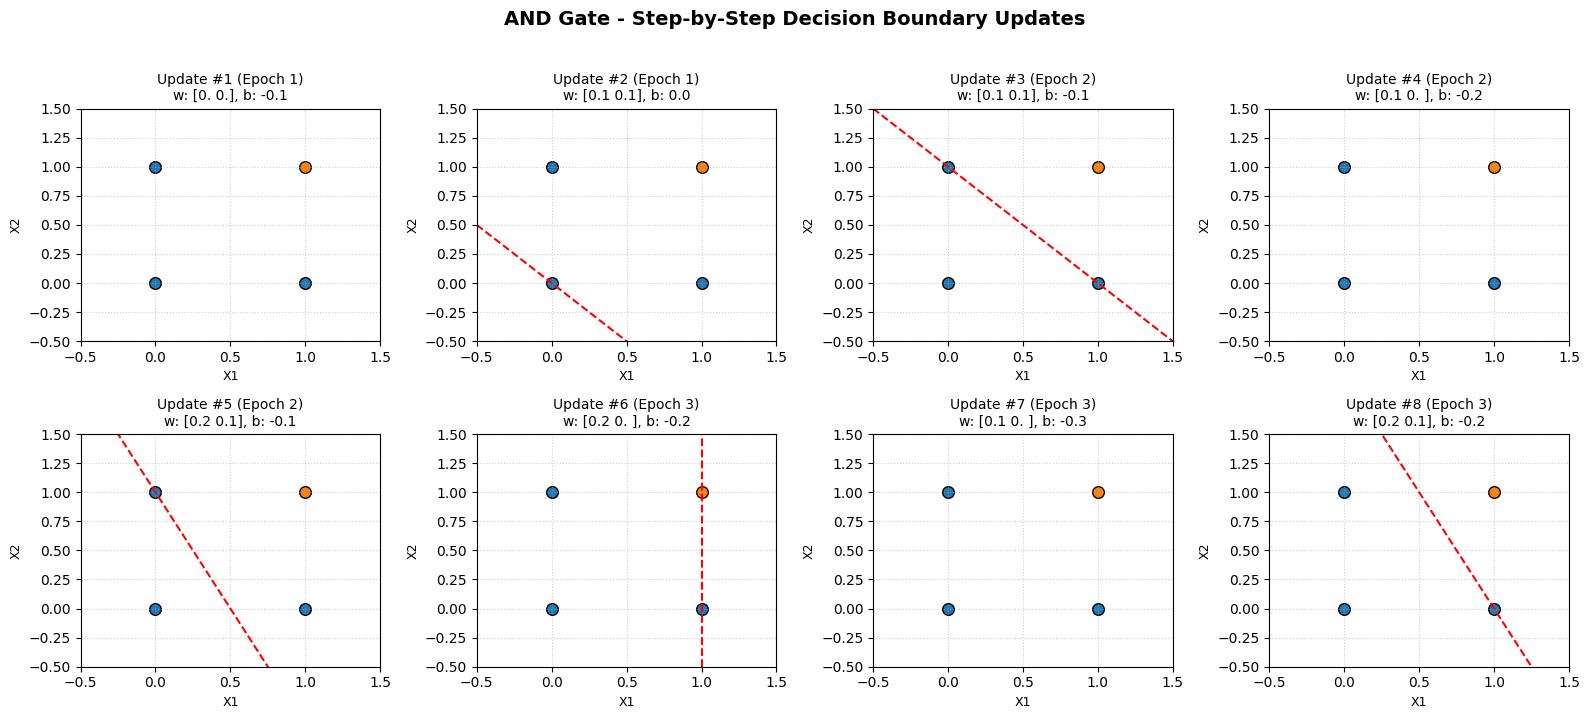
\includegraphics[width=0.85\textwidth]{and_gate_plots.png}
    \caption{Step-by-step decision boundary updates during training of the AND Gate.}
    \label{fig:and_gate_plot}
\end{figure}

\textbf{Inference:} The AND gate requires the strictest threshold since it only outputs $1$ when both inputs are active. The perceptron achieved convergence after 8 updates by driving the bias sufficiently negative ($-0.200$), ensuring that single-active inputs $[0,1]$ and $[1,0]$ fall below the activation threshold.

\vspace{3mm}

% ------------------------------------------------------------------------------
% 2. OR GATE
% ------------------------------------------------------------------------------
\subsection*{OR Gate}

\textbf{Step-by-Step Weight Update Logs}

\begin{center}
\begin{tabular}{|c|c|c|c|c|c|c|}
\hline
Epoch & Update \# & Sample ($x$) & Target ($y$) & Predicted ($\hat{y}$) & New Weights ($w_1, w_2$) & New Bias ($b$)\\
\hline
1 & 1 & $[0,\ 0]$ & 0 & 1 & $[0.000,\ 0.000]$ & $-0.100$\\
\hline
1 & 2 & $[0,\ 1]$ & 1 & 0 & $[0.000,\ 0.100]$ & $0.000$\\
\hline
2 & 3 & $[0,\ 0]$ & 0 & 1 & $[0.000,\ 0.100]$ & $-0.100$\\
\hline
2 & 4 & $[1,\ 0]$ & 1 & 0 & $[0.100,\ 0.100]$ & $0.000$\\
\hline
3 & 5 & $[0,\ 0]$ & 0 & 1 & $[0.100,\ 0.100]$ & $-0.100$\\
\hline
\end{tabular}
\end{center}

\vspace{3mm}

\textbf{OR Gate Summary}

\begin{center}
\begin{tabular}{|p{6cm}|p{7cm}|}
\hline
Convergence Status & Converged at Epoch 4\\
\hline
Total Updates & 5 updates\\
\hline
Final Weights & $[0.100,\ 0.100]$\\
\hline
Final Bias & $-0.100$\\
\hline
\end{tabular}
\end{center}

\begin{figure}[htbp]
    \centering
    % TODO: Replace 'or_gate_plots.png' with your actual plot image filename
    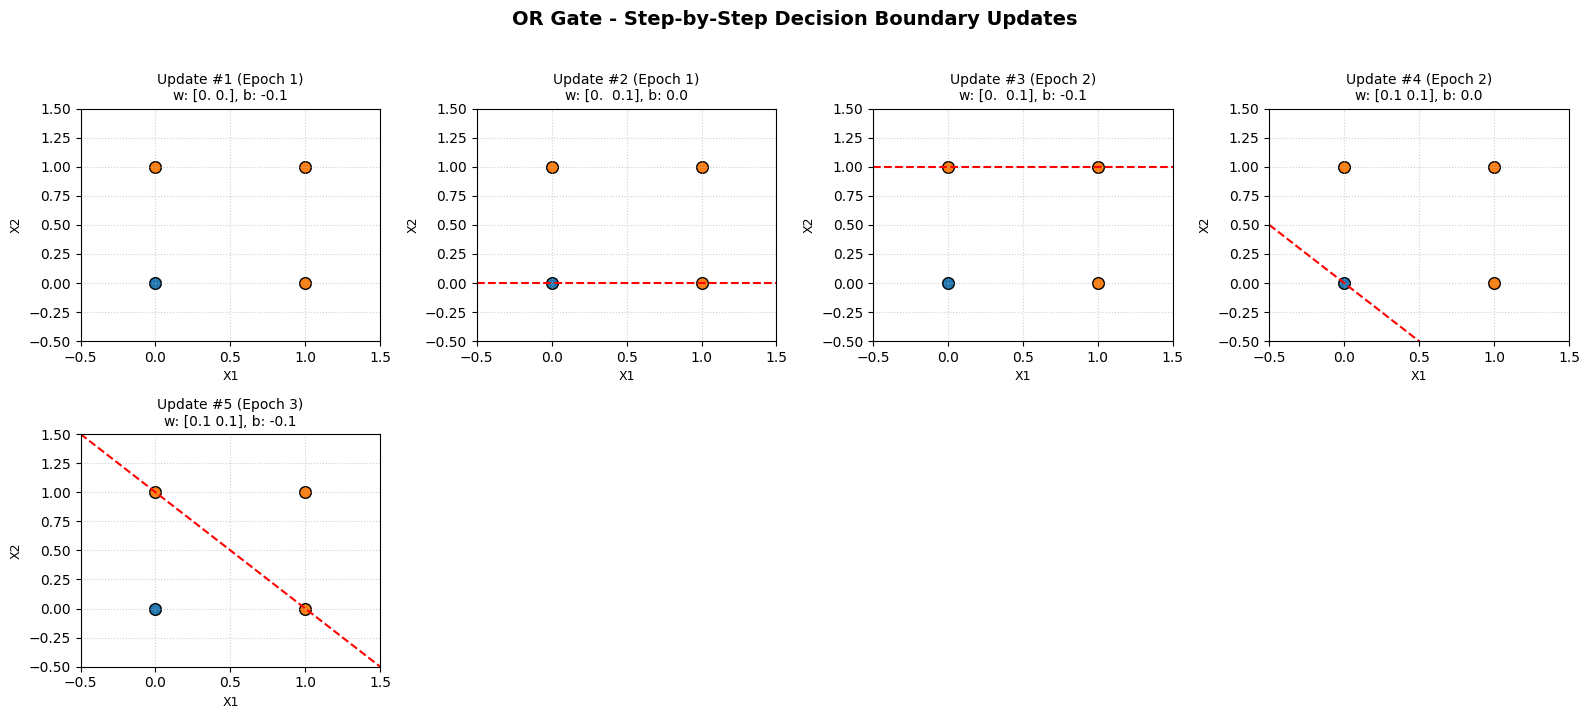
\includegraphics[width=0.85\textwidth]{or_gate_plots.png}
    \caption{Step-by-step decision boundary updates during training of the OR Gate.}
    \label{fig:or_gate_plot}
\end{figure}

\textbf{Inference:} The OR gate converged faster than AND (5 updates vs. 8 updates) because its decision boundary only needs to separate $[0,0]$ from all other points. Equal positive weights ($\mathbf{w} = [0.100, 0.100]$) with a slight negative bias ($-0.100$) allow any input with at least one $1$ to successfully trigger activation.

\vspace{3mm}

% ------------------------------------------------------------------------------
% 3. NOT GATE
% ------------------------------------------------------------------------------
\subsection*{NOT Gate}

\textbf{Step-by-Step Weight Update Logs}

\begin{center}
\resizebox{\textwidth}{!}{%
\begin{tabular}{|c|c|c|c|c|c|c|}
\hline
Epoch & Update \# & Sample ($x$) & Target ($y$) & Pred ($\hat{y}$) & New Weight ($w_1$) & New Bias ($b$)\\
\hline
1 & 1 & $[1]$ & 0 & 1 & $-0.100$ & $-0.100$\\
\hline
2 & 2 & $[0]$ & 1 & 0 & $-0.100$ & $0.000$\\
\hline
\end{tabular}%
}
\end{center}

\vspace{3mm}

\textbf{NOT Gate Summary}

\begin{center}
\begin{tabular}{|p{6cm}|p{7cm}|}
\hline
Convergence Status & Converged at Epoch 3\\
\hline
Total Updates & 2 updates\\
\hline
Final Weights & $[-0.100]$\\
\hline
Final Bias & $0.000$\\
\hline
\end{tabular}
\end{center}

\begin{figure}[htbp]
    \centering
    % TODO: Replace 'not_gate_plots.png' with your actual plot image filename
    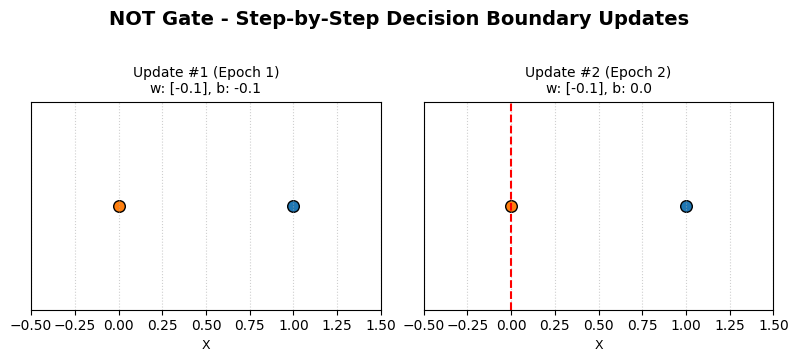
\includegraphics[width=0.85\textwidth]{not_gate_plots.png}
    \caption{Step-by-step decision boundary updates during training of the NOT Gate.}
    \label{fig:not_gate_plot}
\end{figure}

\textbf{Inference:} Being a 1D single-input gate, the NOT gate converged the fastest in just 2 updates across 3 epochs. The learning rule flipped the input weight to negative ($-0.100$), correctly establishing a 1D vertical boundary line at $x = 0$ that inverts $0 \to 1$ and $1 \to 0$.


\clearpage

\section*{11. Discussion}

\textbf{Effect of Learning Rate.} Repeating training with $\eta = 0.001, 0.01, 0.1$ produced identical error curves and identical final test accuracy for all three rates. This is a direct mathematical consequence of the chosen implementation: since the weights and bias are initialized to zero and training samples are processed in the same fixed order every epoch (no shuffling), scaling $\eta$ by a constant only scales the magnitude of the weight vector -- it does not change the \emph{sign} of $\mathbf{w}^T\mathbf{x}+b$ at any step, and therefore does not change which samples are misclassified. This invariance would not hold if the data order were shuffled between epochs or if the weights were randomly initialized.

\vspace{2mm}

\textbf{Step vs.\ Sigmoid Activation.} Step function outputs a constant number and hence gives zero gradient everywhere, making it unsuitable for back-propagation. Whereas, the sigmoid is smooth and differentiable everywhere. Due to this, the Step function is reserved just for classic single layer perceptrons, while deep networks use functions like Sigmoid, ReLU, and Tanh.

\vspace{2mm}

\textbf{Why a Single Layer Perceptron Cannot Solve XOR.} XOR is non-linearly separable. Hence it cannot be separated by a linear decision boundary (a straight line). Therefore, we require at least one hidden layer to add non-linearity to our network and solve the XOR problem.

\vspace{2mm}

\textbf{Effect of Feature Normalization.} Without normalization, features with larger numeric ranges dominate the perceptron's weight updates, since each update is proportional to the raw input value $\mathbf{x}$. Normalizing all features to a comparable scale prevents any single feature from dominating training purely due to its scale, resulting in a more stable and balanced convergence.

\vspace{2mm}

\textbf{From-scratch vs.\ Scikit-learn Perceptron.} The from-scratch implementation achieved a marginally higher test accuracy (0.9891) than scikit-learn's built-in \texttt{Perceptron} (0.9782) on this split. Scikit-learn's \texttt{Perceptron} shuffles training data every epoch and applies an early-stopping criterion, while the from-scratch version iterates over a fixed sample order for a fixed number of epochs; these implementation-level differences lead to slightly different final decision boundaries and, consequently, small accuracy differences on a limited test set.
%----------------------------------------------------------

\section*{12. Conclusion}

A Single Layer Perceptron was implemented entirely from scratch -- including weight/bias initialization, the step activation function, forward propagation, and the perceptron learning rule -- and trained on the Banknote Authentication dataset. After normalization and an 80:20 train--test split, the model's training error dropped sharply within the first few epochs and then plateaued at a low but non-zero level, reflecting that the dataset is close to, but not perfectly, linearly separable. The final model achieved a test accuracy of 98.91\% with perfect precision, confirming that a single linear decision boundary is sufficient to separate the two classes with high reliability. The learning-rate comparison showed that, under this fixed-order, zero-initialized implementation, the choice of $\eta$ affects only the magnitude of the learned parameters and not the classification outcome. Comparison with scikit-learn's \texttt{Perceptron} validated the correctness of the from-scratch implementation, with both models achieving accuracy above 97\%.

%----------------------------------------------------------

\section*{13. References}

\begin{enumerate}
\item F. Rosenblatt, ``The Perceptron,'' \emph{Psychological Review}, 1958.
\item I. Goodfellow, Y. Bengio and A. Courville, \emph{Deep Learning}, MIT Press, 2016.
\item C. M. Bishop, \emph{Pattern Recognition and Machine Learning}, Springer, 2006.
\item S. Haykin, \emph{Neural Networks and Learning Machines}, Pearson, 2009.
\item UCI Machine Learning Repository -- Banknote Authentication Dataset.
\item Scikit-learn Documentation: Perceptron.
\end{enumerate}

\end{document}
